\documentclass[11pt]{article}
\usepackage[T1]{fontenc}
\usepackage{lmodern,microtype,amsmath,amssymb,amsthm,mathtools,booktabs,array,xurl}
\usepackage[a4paper,margin=28mm]{geometry}
\usepackage{tikz}
\usetikzlibrary{arrows.meta,calc,positioning,intersections}
\usepackage[colorlinks=true,linkcolor=blue!55!black,citecolor=blue!55!black,urlcolor=blue!55!black]{hyperref}
\numberwithin{equation}{section}
\setlength{\emergencystretch}{2em}
\newtheorem{theorem}{Theorem}[section]
\newtheorem{proposition}[theorem]{Proposition}
\newtheorem{lemma}[theorem]{Lemma}
\newtheorem{corollary}[theorem]{Corollary}
\theoremstyle{definition}\newtheorem{definition}[theorem]{Definition}
\theoremstyle{remark}\newtheorem{remark}[theorem]{Remark}
\newcommand{\ii}{\mathrm i}
\newcommand{\dd}{\mathrm d}
\newcommand{\Vol}{\operatorname{Vol}}
\newcommand{\Rea}{\operatorname{Re}}
\newcommand{\Ima}{\operatorname{Im}}
\newcommand{\Log}{\operatorname{Log}}
\newcommand{\diag}{\operatorname{diag}}
\newcommand{\Turn}{\mathsf T}
\newcommand{\eps}{\varepsilon}
\newcommand{\CC}{\mathbb C}
\newcommand{\RR}{\mathbb R}
\newcommand{\kap}{\varkappa}
\title{Marked geometry of strict Conway compositions}
\author{}\date{}
\begin{document}\maketitle
\begin{abstract}
An ordered expression in crossing-circle tangles, products and physical
turns determines a link diagram and a real wire polytope. We construct
the complete hyperbolic metric whenever that polytope has a strict state.
Four separate boundary-edge labels allow the pyramid-and-prism
construction to pass through turned elementary children and arbitrary
strict closing pairs. We prove convexity, retain every original shaded
triangle, and identify the closed assembly with the literal projection
cut of the specified link. Whole complex face maps then give its marked
deformation, with parabolic main cusps. The original primitive filling
equations have a unique small solution for independently long signed
slopes. Smooth completion and an absolute fundamental-chain comparison
identify the volume with a critical value of a classical cell potential.
No asymptotic formula for a quantum invariant is used or asserted.
\end{abstract}

\section{The fixed diagram and the geometric statements}\label{sm:intro}

A crossing circle is an auxiliary unknotted component bounding a disk
punctured twice by the main strands. We retain its disk and its original
framing. Let $h$ be the physical quarter-turn of this elementary
two-strand tangle, with full twists removed. A construction is a finite
expression in distinct copies of $h$, ordered products and physical
clockwise quarter-turns $\Turn$. No reduced algebraic expression replaces
the original diagram in this paper.

The four endpoints of a box are numbered $0,1,2,3$ cyclically, starting
at the bottom left. In the stack $FG$, with $F$ below $G$, join
$F_2$ to $G_1$ and $F_3$ to $G_0$. Its exposed tuple is
$(F_0,F_1,G_2,G_3)$. A turn replaces a tuple by
$(C_1,C_2,C_3,C_0)$ and moves the entire box and all its disks.
Cylindrical closure $C$ joins endpoints $0$ to $3$ and $1$ to $2$.
Our closed diagrams are $C(FG)$ with arbitrary such $F,G$ subject to
the following condition.

\begin{definition}\label{sm:strict}
A strict wire state assigns a leaf variable $a\in(0,1/2)$ and an
output variable to every open subexpression. A turn complements its
variable. Every product retained below the closing root satisfies
\begin{equation}\label{sm:gate-domain}
             \max(x,y)<z<x+y<1.
\end{equation}
The two closing outputs are $b,1-b$. The final forced gate is removed,
but this complementary relation is retained. An expression is strict
if the resulting real polytope has a strict state.
\end{definition}

Thus strictness is a condition on this particular presentation. A turned
leaf or a bare leaf may occur at a closing child. This is larger syntax
than the completed/completed closing grammar of \cite{Geometry}; its
global metric theorem will not be applied here.

Fix $\eps_i\in\{-1,0,1\}$ at the $H$ original leaves. It specifies
the retained signed half twist; $\eps_i=0$ is the pure disk pairing.
Let $Y_E^\eps$ be the exterior in $S^3$ of the resulting augmented
link, retaining all $H$ crossing circles and every main component.
The source-independent functions used below are
\begin{align}
 J(u)&=\int_0^u\log(2\sin\pi t)\,\dd t\quad(0\le u\le1),
       &J(1-u)&=-J(u),\label{sm:J}\\
 g(a)&=J(2a)-4J(a),\label{sm:g}\\
 m(x,y,z)&=J(x+y)+J(z)-J(x)-J(y)\notag\\
 &\hspace{13mm}-J(z-x)-J(z-y)-J(x+y-z).\label{sm:m}
\end{align}
Let $\mathcal F$ be the sum of $g$ over leaves and $m$ over retained
products, and let $F_0$ denote its maximum. The variational theorem
of \cite{Profiles} supplies the unique strict optimizer and its
negative definite Hessian in independent wires. We state the precise
input in Section~\ref{sm:variational}; its proof does not use a
global metric or a quantum noncancellation theorem.

\begin{theorem}[Complete marked exterior]\label{sm:complete}
For every fixed strict expression and retained half-twist pattern,
$Y_E^\eps$ has a complete finite-volume hyperbolic metric assembled
from two copies of a convex right-angled ideal polyhedron. Its volume is
\begin{equation}\label{sm:complete-volume}
                     \Vol(Y_E^\eps)=2\pi F_0.
\end{equation}
At each crossing circle the original meridian $\mu_i$ and disk
longitude $\lambda_i$ are a primitive ordered basis. Their complete
longitude-to-meridian translation ratio is
\begin{equation}\label{sm:tau}
 \tau_i=\frac{2\ii c_i}{1-\eps_i\ii c_i},\qquad
 c_i=\cot(\pi a_i)>0,\qquad \Ima\tau_i>0.
\end{equation}
All original main components have complete cusp ends.
\end{theorem}

The primitive basis fixes the filling convention. For a subset
$I\subseteq\{1,\ldots,H\}$ and integers $p_i$, fill precisely the
auxiliary slopes $\mu_i+p_i\lambda_i$, $i\in I$. Denote the original
filled exterior by $Y_E^\eps(\mathbf p;I)$. Cutting the original disk,
rotating through $p_i$ full turns and removing its crossing circle
inserts the physical power $\eps_i-2p_i$ in that same disk frame.
The disjoint disk neighborhoods show directly that the ambient manifold
is still $S^3$. We never fill a main cusp.

\begin{theorem}[Primitive signed fillings]\label{sm:fillings}
There is a holomorphic classical potential $\Phi_\eps(\boldsymbol\chi)$,
with $\Phi_\eps(0)=F_0$, and a framed representation of the original
group near its oriented complete holonomy, whose primitive similarity
logarithms are
\begin{equation}\label{sm:UV}
       U_i=-2\pi\ii\chi_i,\qquad V_i=-2\partial_i\Phi_\eps.
\end{equation}
Every main peripheral group remains parabolic. Set $\chi_i=0$ outside
$I$. There is a bound $B_{E,\eps,I}$ such that, whenever all
$|p_i|>B_{E,\eps,I}$, the restricted action
\begin{equation}\label{sm:filled-action}
 S_{\eps,\mathbf p}(\boldsymbol\chi)=\Phi_\eps(\boldsymbol\chi)
       +\frac{\pi\ii}{2}\sum_{i\in I}\frac{(\chi_i-1)^2}{p_i}
\end{equation}
has a unique critical point in a fixed neighborhood of zero. The
representation there completes to a smooth complete finite-volume
hyperbolic metric on the original $Y_E^\eps(\mathbf p;I)$, and
\begin{equation}\label{sm:filled-volume}
 \Vol\bigl(Y_E^\eps(\mathbf p;I)\bigr)
                   =2\pi\Rea S_{\eps,\mathbf p}(\boldsymbol\chi_*).
\end{equation}
The signs and relative sizes of the filling integers are independent.
If $I$ contains all auxiliaries and the literal strand pairing has one
component, the right side is the volume of that knot complement.
\end{theorem}

The uniqueness assertion is local in this prescribed family, not a
classification of the character variety. The potential is defined from
the cells in Section~\ref{sm:potential}; no selected quantum action is
an input. A maximum over the finitely many $\eps,I$ gives one bound
for a fixed strict expression if desired. An empty filling subset
recovers Theorem~\ref{sm:complete}.

The classical geometry of fully augmented links and their half-twist
partners is well established; see \cite{Purcell}. Dehn filling and
holomorphic peripheral potentials belong to the framework of
\cite{NZ}. The work here is the ordered individual-edge assembly and
its marked continuation for strict expressions, with the original
manifold and the absolute normalization proved explicitly.

\section{Variational input and local cells}\label{sm:variational}

We use the following specific conclusions of the strict-profile
companion \cite[Lemma~2.2, Theorem~3.3, Lemma~4.1 and
Proposition~4.2]{Profiles}.
For each nonempty strict fixed-output domain, the maximum over the
internal wires is strict, unique and nondegenerate. Its profile $f_E(b)$
is real analytic on that domain. The analogous closed statement holds
on Definition~\ref{sm:strict}'s reduced affine constraint space.
The exact open types and product table are
\begin{equation}\label{sm:types}
 L=(0,1/2),\quad H=(1/2,1),\quad A=(0,1),\qquad
 \begin{array}{c|ccc}
    &L&H&A\\\hline
 L&A&H&A\\ H&H&\varnothing&H\\ A&A&H&A
 \end{array}.
\end{equation}
Every point of each indicated interval is attained. A leaf has type
$L$; a turn exchanges $L,H$ and preserves $A$. The nonempty closing
pairs are $AA,AL,AH,LH$ and their reversals.

For an optimized output define
\begin{equation}\label{sm:profile-data}
 B=\cot\pi b,\quad \kap=e^{-f_E'(b)},\qquad
 X^2=\frac{1+B^2}{1+\kap},\quad Y^2=\kap X^2,
 \quad X,Y>0.
\end{equation}
Then $X^2+Y^2-B^2=1$, and the imported profile identities give
\begin{equation}\label{sm:profile-types}
 L:(B,X,Y)=(B,B,1),\qquad H:(B,X,Y)=(-Y,1,Y),
 \qquad A:-Y<B<X.
\end{equation}
A turn sends $(B,X,Y)$ to $(-B,Y,X)$. At a stationary product the
two children have a common $X$, and, writing $S=B_1+B_2>0$,
\begin{equation}\label{sm:profile-product}
       B_o=\frac{B_1B_2+X^2-1}{S},\qquad
       Y_o=\frac{Y_1Y_2}{S}.
\end{equation}
These are scalar variational identities; they do not identify an
open quadrilateral with a physical four-punctured tangle boundary.

\subsection{The ideal-tetrahedron normalization}
\label{sm:local-cells}

We use upper half-space with ideal boundary
$\CC\cup\{\infty\}$. A geodesic plane is vertical over a line or
is a hemisphere orthogonal to the boundary plane. A horizontal
horosphere at $\infty$ has a Euclidean induced metric up to scale.
For positive $a,b,c$ with $a+b+c=1$, the classical volume of
an ideal tetrahedron with dihedral angles $\pi a,\pi b,\pi c$ is
\begin{equation}\label{sm:tetra}
 \begin{split}
 V(a,b,c)&=\Lambda(\pi a)+\Lambda(\pi b)+\Lambda(\pi c)
              =-\pi\{J(a)+J(b)+J(c)\},\\
 \Lambda(t)&=-\int_0^t\log(2\sin u)\,\dd u .
 \end{split}
\end{equation}
We import this normalized local formula, including its continuous
zero value at a flat tetrahedron, from classical hyperbolic
geometry \cite{Milnor}. All cell volumes below are ordinary sums
of positive tetrahedron volumes.

\subsection{The leaf pyramid}
For $0<a<1/2$, put $E=e^{2\pi\ii a}$. The convex hull of
\begin{equation}\label{sm:leaf}
 O=\infty,\qquad (C_0,C_1,C_2,C_3)=(1,E,-1,-E)
\end{equation}
is an ideal quadrangular pyramid. Its four finite vertices form
a rectangle. Its side planes are vertical over the four rectangle
edges; its base plane is the unit hemisphere. These five
supporting planes enclose exactly the convex hull. Adjacent
vertical planes meet at right angles, so every apex edge has
angle $\pi/2$.

Call base edges $01,23$ free and $12,30$ cap edges. Intersecting
a vertical chord plane with the unit hemisphere gives interior
angle equal to half the angle subtended by that chord at the
circle center. Thus free edges have angle $\pi a$, and cap
edges have angle $\pi(1/2-a)$.
Color $(O,C_1,C_2)$ and $(O,C_3,C_0)$ shaded and the other two
side triangles white. The shaded faces will retain the two
sides of the original half crossing disk. The ordered
quadrilateral base is a gluing face in the cut construction.

The diagonal $C_0C_2$ divides the pyramid into two positive
tetrahedra with angle triple $(a,1/2-a,1/2)$. By
\eqref{sm:tetra},
\[
 \Vol(\text{leaf})=2V(a,1/2-a,1/2)=\pi g(a).
\]
The last equality follows either by differentiating the two
expressions and evaluating at $a=0$, or from
$J(2a)=2J(a)-2J(1/2-a)$.

\begin{figure}[ht]
\centering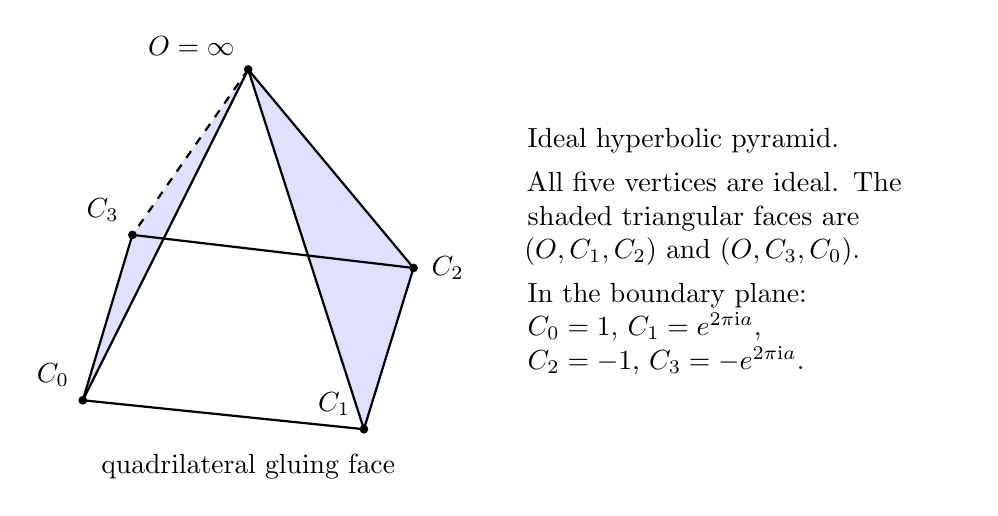
\begin{tikzpicture}[scale=1.05]
\coordinate (c0) at (-2,-1);\coordinate(c1) at (1.4,-1.35);\coordinate(c2) at (2,.6);\coordinate(c3) at (-1.4,1);\coordinate(o) at (0,3);
\fill[blue!12] (o)--(c1)--(c2)--cycle;\fill[blue!12] (o)--(c3)--(c0)--cycle;
\draw[thick] (c0)--(c1)--(c2)--(c3)--cycle;
\draw[thick] (o)--(c0) (o)--(c1) (o)--(c2);\draw[thick,dashed] (o)--(c3);
\foreach \p/\l in {c0/C_0,c1/C_1,c3/C_3,o/O=\infty}{\fill (\p) circle(1.5pt);\node[above left=2pt] at (\p) {$\l$};}
\fill (c2) circle(1.5pt);\node[right=3pt] at (c2) {$C_2$};
\node at (0,-1.8) {quadrilateral gluing face};
\node[align=left,text width=5.5cm] at (6,.8) {Ideal hyperbolic pyramid.\\[4pt]All five vertices are ideal. The shaded triangular faces are $(O,C_1,C_2)$ and $(O,C_3,C_0)$.\\[4pt]In the boundary plane:\\ $C_0=1$, $C_1=e^{2\pi\ii a}$,\\ $C_2=-1$, $C_3=-e^{2\pi\ii a}$.};
\end{tikzpicture}

\caption{The ideal hyperbolic leaf pyramid. The two shaded
triangles record the sides of a half crossing disk. The ordered
quadrilateral is a gluing face of the cut cells; it is not
identified with the physical four-punctured boundary of a
tangle box.}\label{sm:leaf-figure}
\end{figure}

\subsection{The multiplication prism}
Given a strict product, put
$p=z-x$, $q=z-y$, $r=x+y-z$, $w=1-x-y$.
All four numbers are positive, and $p+q+2r+w=1$.
Choose four points on the unit circle:
\begin{equation}\label{sm:prism-vertices}
 v_0=1,\qquad v_1=e^{2\pi\ii p},\qquad
 v_2=e^{2\pi\ii(p+r)},\qquad
 v_3=e^{2\pi\ii(p+r+q)}.
\end{equation}
Their successive half-arcs are $p,r,q,r+w$.
The extended chords $v_0v_1$ and $v_3v_2$ meet at a point $P$.
The triangle $(P,v_1,v_2)$ has angles $\pi w,\pi y,\pi x$
at those respective vertices. The sine rule, with chord lengths
$2\sin\pi p$, $2\sin\pi q$, $2\sin\pi r$, gives
\begin{equation}\label{sm:prism-P}
 \begin{split}
 P&=v_1+
 \frac{\sin\pi x\sin\pi r}{\sin\pi w\sin\pi p}(v_1-v_0)\\
  &=v_2+
 \frac{\sin\pi y\sin\pi r}{\sin\pi w\sin\pi q}(v_2-v_3).
 \end{split}
\end{equation}
Both coefficients are positive. Thus the orders on the two
lines are $v_0,v_1,P$ and $v_3,v_2,P$.

Attach the tetrahedron $(\infty,P,v_1,v_2)$ to the pyramid
$(\infty,v_0,v_1,v_2,v_3)$ across $(\infty,v_1,v_2)$.
Their interiors lie on opposite sides of that vertical plane.
The faces over $v_0v_1$ and $v_1P$ are coplanar, as are those
over $v_3v_2$ and $v_2P$. Merging them leaves three quadrilateral
faces and two triangular faces:
\[
 \begin{gathered}
 F_x=(\infty,v_0,v_1,P),\qquad
 F_y=(\infty,v_3,v_2,P),\qquad F_z=(v_0,v_1,v_2,v_3),\\
 (P,v_1,v_2),\qquad(\infty,v_0,v_3).
 \end{gathered}
\]
The last two faces are white.

There are five supporting planes: the vertical planes over
$v_0v_1$, $v_2v_3$, $v_3v_0$, and the hemispheres over the
circles $(v_0,v_1,v_2,v_3)$ and $(P,v_1,v_2)$.
The power of $P$ with respect to the unit circle is positive,
because $P$ is beyond $v_1$ on the chord $v_0v_1$.
Likewise the powers of $v_0,v_3$ with respect to the circle
$(P,v_1,v_2)$ are positive: along its two secants the points
have orders $v_0,v_1,P$ and $v_3,v_2,P$.
Consequently both attached pieces are in the same inward
half-space of each of these five planes. Their union is the
convex ideal triangular prism bounded by those faces.
This proves support and nonintersection throughout the strict
domain, rather than for one drawn example.

\begin{figure}[ht]
\centering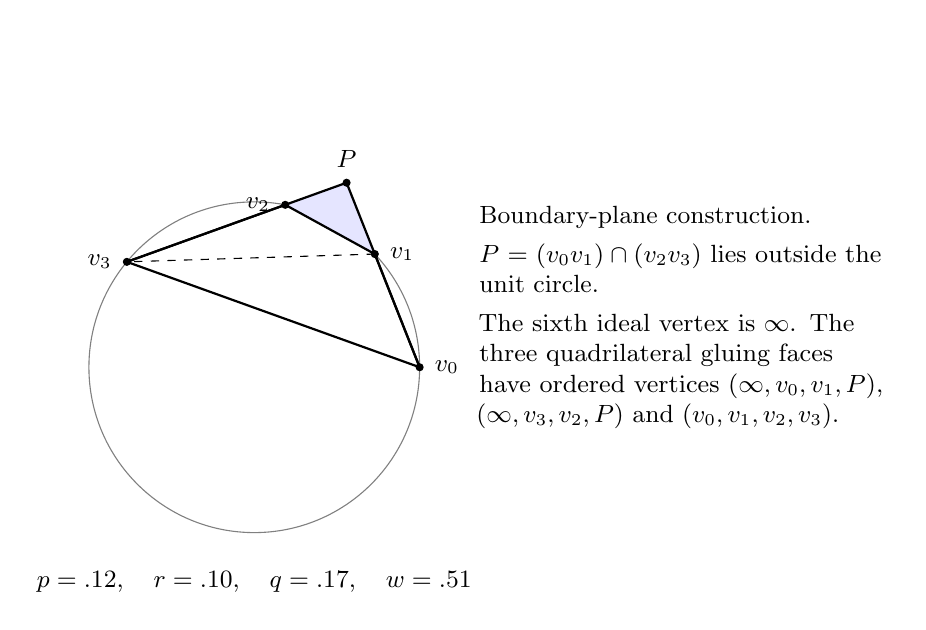
\begin{tikzpicture}[scale=2.1, every node/.style={font=\small}]
\coordinate(v0) at (1,0);
\coordinate(v1) at ({cos(43.2)},{sin(43.2)});
\coordinate(v2) at ({cos(79.2)},{sin(79.2)});
\coordinate(v3) at ({cos(140.4)},{sin(140.4)});
\coordinate(P) at (0.57935,1.06242);
% Exact intersection of the two extended chords is used below.
\path[name path=first] (v0)--($(v0)!3!(v1)$);
\path[name path=second] (v3)--($(v3)!3!(v2)$);
\path[name intersections={of=first and second,by=P}];
\draw[gray] (0,0) circle(1);
\fill[blue!10] (P)--(v1)--(v2)--cycle;
\draw[thick] (v0)--(P)--(v3)--cycle;
\draw[thick] (v0)--(v1)--(v2)--(v3);
\draw[dashed] (v1)--(v3);
\foreach \p/\lab/\pos in {v0/v_0/right,v1/v_1/right,v2/v_2/left,v3/v_3/left,P/P/above}
 {\fill (\p) circle(.7pt);\node[\pos=2pt] at(\p){$\lab$};}
\node at (0,-1.3) {$p=.12,\quad r=.10,\quad q=.17,\quad w=.51$};
\node[align=left,text width=5.2cm] at (2.6,.3) {Boundary-plane construction.\\[3pt]$P=(v_0v_1)\cap(v_2v_3)$ lies outside the unit circle.\\[3pt]The sixth ideal vertex is $\infty$. The three quadrilateral gluing faces have ordered vertices $(\infty,v_0,v_1,P)$, $(\infty,v_3,v_2,P)$ and $(v_0,v_1,v_2,v_3)$.};
\end{tikzpicture}

\caption{Boundary-plane support data for the multiplication
prism; its sixth ideal vertex is $\infty$. The point $P$ is
the intersection of the extended chords, with the two orders
proved in \eqref{sm:prism-P}. The circle through $P,v_1,v_2$
and the unit circle support the two bounded faces.}
\label{sm:prism-figure}
\end{figure}

The original lower and upper attachments and the output order are
\begin{equation}\label{sm:stack-map}
 F:C\mapsto(v_0,v_1,P,\infty),\quad
 G:C\mapsto(\infty,P,v_2,v_3),\quad
 C^o=(v_0,v_1,v_2,v_3).
\end{equation}
Reading angles between the supporting planes gives
\begin{equation}\label{sm:prism-angles}
\begin{array}{c|ccccc}
\text{edge}&Pv_1,\infty v_0&Pv_2,\infty v_3&
v_1v_2,v_0v_3&P\infty&v_0v_1,\ v_2v_3\\\hline
\text{angle}/\pi&x&y&1-z&w&p,\ q
\end{array}.
\end{equation}
For a circle and a chord plane, the dihedral angle is the
opposite inscribed angle. Applied to $(P,v_1,v_2)$ this gives
$x,y$ at $Pv_1,Pv_2$; the angle between the two vertical chord
planes is $\pi w$. At the unit-circle base the half-arcs give
$p,q$. The remaining angles follow at the ideal vertices:
their Euclidean links are triangles, so the interior dihedral
angles sum to $\pi$. For example $x+y+w=1$ at $P$, and
$x+p+(1-z)=1$ at $v_1$. This verifies every row of the table.

Divide the original quadrangular pyramid across $v_0v_2$.
Its tetrahedron triples are $(p,r,1-p-r)$ and
$(p+r,q,r+w)$. In their volumes the terms at $p+r$ and
$1-p-r$ cancel. The attached tetrahedron has triple $(y,x,w)$.
Thus the sum is also
\begin{equation}\label{sm:prism-volume}
 \begin{split}
 \Vol(\text{prism})
 &=V(y,x,w)+V(p,q,2r+w)+V(p+q,r,r+w)\\
 &=\pi m(x,y,z).
 \end{split}
\end{equation}
To check the first rewriting, the two extra terms
$\Lambda(\pi(p+q))$ and $\Lambda(\pi(2r+w))$ cancel because
their arguments sum to $\pi$. For the second equality use
$x=q+r$, $y=p+r$, $z=p+q+r$, $r+w=1-z$ and
$w=1-x-y$ in \eqref{sm:tetra}. All triples used here are
positive and sum to one.

\subsection{Matching the whole ordered face}
For a cyclically ordered ideal quadruple define
\begin{equation}\label{sm:kappa}
 \kap(a,b,c,d)=\frac{(a-b)(c-d)}{(a-d)(b-c)}>0
\end{equation}
with the usual limits at infinity. Sending three vertices
to $(\infty,0,1)$ shows that this positive number determines
the entire ordered ideal quadrilateral, including its shear.
A one-step cyclic shift and a reversal fixing the first
vertex invert $\kap$; full reversal preserves it.

Formula \eqref{sm:prism-P} immediately gives the first two
ratios below as directed ratios on the chord lines; the
third follows from the four unit-circle chord lengths:
\begin{align}
 \kap(F_x)&=\frac{\sin\pi x\sin\pi r}
                    {\sin\pi w\sin\pi p}=e^{-m_x},&
 \kap(F_y)&=\frac{\sin\pi y\sin\pi r}
                    {\sin\pi w\sin\pi q}=e^{-m_y},\label{sm:input-kappa}\\
 \kap(F_z)&=\frac{\sin\pi p\sin\pi q}
                    {\sin\pi z\sin\pi r}=e^{-m_z}.&&\label{sm:output-kappa}
\end{align}
The derivative equalities follow by differentiating the seven
$J$ terms in \eqref{sm:m}; for example
$m_x=\log(\sin\pi w\sin\pi p/(\sin\pi x\sin\pi r))$.
The leaf ratio is $\tan^2(\pi a)=e^{-g'(a)}$.

The lower tuple in \eqref{sm:stack-map} is a cyclic shift of
$F_x$ and the upper is a reversal fixing the first vertex of
$F_y$, so both invert the input ratios. The stationary equations
$f_F'(x)+m_x=0$ and $f_G'(y)+m_y=0$ therefore match all four
ordered vertices of each attachment. The output derivative is
$m_z$, which proves $\kap=e^{-f_E'}$ inductively.
A physical turn cyclically relabels the quadruple and replaces
$b$ by $1-b$, again inverting the ratio.
Finally $C_j^F\mapsto C_{3-j}^G$ is full reversal.
The closing equation $f_F'(b)=f_G'(1-b)$ therefore matches the
whole closing face. None of these steps replaces a complex
shape by its absolute value.


\section{Four boundary labels and convex assembly}\label{sm:masks}

An open cell has one ordered quadrilateral gluing face
$Q=(C_0,C_1,C_2,C_3)$. Number its edges $j=(j,j+1)$ modulo four.
Edges $0,2$ are called free, and $1,3$ cap edges. These names record
the original leaf order, not an unmarked symmetry of the whole tangle.
Set $\eta_j=1$ if the face beside edge $j$, other than $Q$, is shaded,
and set $\eta_j=0$ if it is white. The four bits
$\boldsymbol\eta=(\eta_0,\eta_1,\eta_2,\eta_3)$ will be called the
boundary mask.

\begin{proposition}\label{sm:mask-invariant}
At every open subexpression evaluated at its strict stationary wires
there is a convex ideal cell with a maximal, nondegenerate ordered
quadrilateral output. Its boundary-edge angles are
\begin{equation}\label{sm:masked-angles}
 \frac{\theta_j}{\pi}=
 \begin{cases}
 b-\eta_j/2,&j=0,2,\\
 1-b-\eta_j/2,&j=1,3.
 \end{cases}
\end{equation}
Every other surviving edge is right angled and separates a white
face from a shaded triangle. The possible supports satisfy
\begin{equation}\label{sm:mask-support}
 L:\eta_0=\eta_2=0,\qquad H:\eta_1=\eta_3=0,\qquad
 A:\boldsymbol\eta=0.
\end{equation}
Every original shaded triangle remains an entire face. The four
output corners are four active original terminal singletons.
Every other main ideal vertex is a permanently consumed pair of
terminals; crossing-circle apices stay separate.
\end{proposition}

The statement permits a type $H$ output with only one shaded free
edge. Replacing its two free angles by a common angle would therefore
lose information essential to the next gluing.

\begin{figure}[ht]
\centering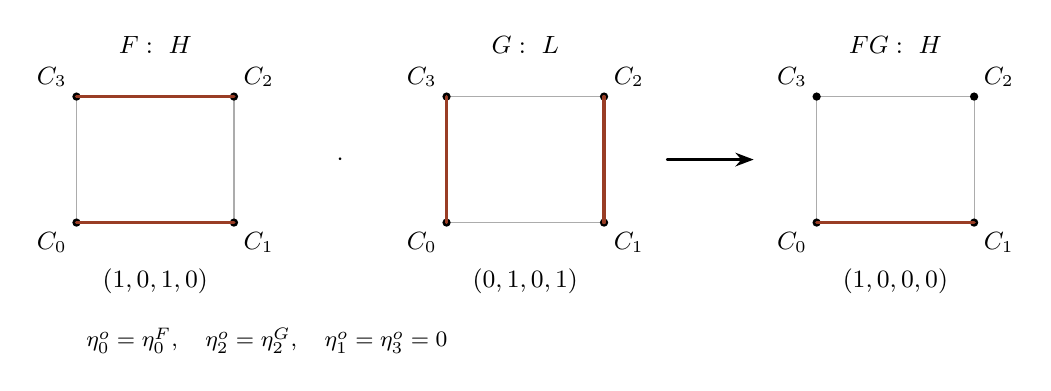
\begin{tikzpicture}[x=1cm,y=1cm,line cap=round,
  every node/.style={font=\small},>=Stealth]
 \definecolor{shadeedge}{RGB}{153,61,37}
 \foreach \x/\title/\bits in {0/$F:\ H$/{},4.7/$G:\ L$/{},9.4/$FG:\ H$/{}} {
  \begin{scope}[shift={(\x,0)}]
   \coordinate (a) at (0,0);
   \coordinate (b) at (2,0);
   \coordinate (c) at (2,1.6);
   \coordinate (d) at (0,1.6);
   \draw[gray!65] (a)--(b)--(c)--(d)--cycle;
   \foreach \p/\lab/\pos in {a/0/below left,b/1/below right,c/2/above right,d/3/above left}
    {\fill (\p) circle (1.5pt); \node[\pos] at (\p) {$C_{\lab}$};}
   \node at (1,2.25) {\title};
  \end{scope}
 }
 \draw[shadeedge,very thick] (0,0)--(2,0) (0,1.6)--(2,1.6);
 \draw[shadeedge,very thick] (4.7,0)--(4.7,1.6) (6.7,0)--(6.7,1.6);
 \draw[shadeedge,very thick] (9.4,0)--(11.4,0);
 \node at (1,-.75) {$(1,0,1,0)$};
 \node at (5.7,-.75) {$(0,1,0,1)$};
 \node at (10.4,-.75) {$(1,0,0,0)$};
 \node at (3.35,.8) {$\cdot$};
 \draw[->,thick] (7.5,.8)--(8.6,.8);
 \node[anchor=west,font=\footnotesize] at (0,-1.5)
 {$\eta^o_0=\eta^F_0,\quad \eta^o_2=\eta^G_2,\quad
   \eta^o_1=\eta^o_3=0$};
\end{tikzpicture}

\caption{Individual boundary labels in an $HL$ product. A colored
edge has a shaded adjacent face; the other edges have a white
adjacent face. The turned leaf has mask $(1,0,1,0)$, the upper
leaf has mask $(0,1,0,1)$, and the product has mask $(1,0,0,0)$.
Its two free angles are $\pi(z-1/2)$ and $\pi z$.
The pictures display the ordered quadrilateral gluing faces.}
\label{sm:mask-figure}
\end{figure}

\subsection{Every seam angle}
For a leaf the mask is $(0,1,0,1)$, so
\eqref{sm:masked-angles} is the pyramid angle calculation.
A turn rotates the mask by one and replaces $b$ by $1-b$.
This proves the assertion under turns and exchanges the support
conditions for $L,H$.

At a product the output mask is exactly
\begin{equation}\label{sm:mask-product}
         \boldsymbol\eta^o=(\eta^F_0,0,\eta^G_2,0).
\end{equation}
Indeed the two output cap sides adjoin the prism's white triangles,
and each output free side inherits its indicated child side.
A child cap seam has angle
$\pi(1-\eta_j/2)$: a zero bit merges two white pieces flatly, while
a one bit leaves a right shaded--white edge.
At the edge common to both prism inputs, the total angle is
\begin{equation}\label{sm:shared-angle}
 \pi\left[w+x-\frac{\eta^F_2}{2}
             +y-\frac{\eta^G_0}{2}\right]
       =\pi\left[1-\frac{\eta^F_2+\eta^G_0}{2}\right].
\end{equation}
Both bits could be one only with two type $H$ inputs, forbidden
by \eqref{sm:types}. Thus this seam is either flat white--white
or right shaded--white. The remaining free output angles are
$\pi(p+x-\eta^F_0/2)$ and $\pi(q+y-\eta^G_2/2)$; the cap
angles are $\pi(1-z)$. This gives \eqref{sm:masked-angles}.

The support assertion also follows case by case from
\eqref{sm:types}. An output of type $A$ has no type $H$ child,
so both inherited free bits vanish. An output of type $H$ has
zero cap bits by \eqref{sm:mask-product}. Turns give all type $L$
cases. We assert these support inclusions, not equality with the
two-bit leaf masks.

For successive convex attachments one must check the intermediate
stage, not only the final totals. Attach $F$ to the prism first.
Its free seams have angles
\[
 \pi(z-\eta^F_0/2),\qquad
 \pi(1-y-\eta^F_2/2).
\]
If the first bit is one, $F$ has type $H$, hence $z>x>1/2$.
If the second bit is one, $x>1/2$ and $x+y<1$ give $y<1/2$.
Both displayed angles are therefore positive and strictly less
than $\pi$. In particular the other prism input remains a
supported nondegenerate quadrilateral. The cap seams have already
been checked. The second attachment is now justified by
\eqref{sm:shared-angle}.

\subsection{Convexity includes the ideal boundary}
Here is the geometric argument used at each attachment. Place two
convex finite-faced ideal polyhedra on opposite sides of the plane
of the matched quadrilateral. Their finite intersection is that
face. The finite union is closed, connected and locally convex:
the only new boundary points lie on the seam edges, where the
total angle is at most $\pi$. There are no finite seam vertices.

Two finite points in the union have a shortest path in it.
Indeed a length-bounded minimizing sequence stays in a compact
ambient hyperbolic ball. Constant-speed parametrization and
Arzelà--Ascoli give a limiting path; closedness keeps it in the
union. Local convexity makes each small subarc the ambient
geodesic. The complete path is therefore the unique ambient
geodesic segment. This proves convexity of the union.

There is a further ideal-point issue. The two ideal closures can
meet only on the boundary circle of the common supporting plane.
The intersection of either cell with that plane is exactly its
maximal quadrilateral face. An additional ideal vertex on the
circle would enlarge that face past one of its edges, making the
edge flat; all four supporting angles there are strictly nonflat.
Equivalently, in the Klein model the closed quadrilateral meets
the sphere at infinity only in its four vertices. Thus the only
ideal coincidences are the four specified corner identifications.
This argument applies again to the second input, which the
intermediate angle check kept strictly supported.

Every output angle in \eqref{sm:masked-angles} lies in $(0,\pi)$
on its actual type interval. Hence the output remains a maximal
supported quadrilateral and the induction continues. Every
shaded-triangle seam is right, never flat. Only white faces merge:
no shaded edge or triangle is deleted, split or merged with
another shaded face. A leaf apex is never in an attaching
quadrilateral. It retains its four right edges and its two
original shaded sectors.

\subsection{Terminal pairs never become chains}
Give leaf $i$ the four distinct terminal symbols $(i,0),\ldots,(i,3)$
and the distinct apex symbol $O_i$. The purely literal endpoint
rules prove the following invariant independently of the metric.
An open expression has four active singleton terminals; all other
terminals form disjoint consumed two-element pairs. A turn only
permutes the active tuple. Product consumes exactly
\begin{equation}\label{sm:terminal-product}
          F_2\sim G_1,\qquad F_3\sim G_0,
\end{equation}
and keeps $F_0,F_1,G_2,G_3$ active. The child leaf sets are disjoint.
A consumed pair is never subsequently attached or exposed.
Thus no class grows to three terminals. The geometric maps
\eqref{sm:stack-map} make exactly these pairs; the ideal-point
argument excludes any additional identification.

At an exposed corner the two adjacent mask bits have sum at most one.
If their sum is zero, its cyclic faces are the gluing quadrilateral,
white, shaded, white; if the sum is one there are only the
quadrilateral, white and shaded faces in the retained order.
This also follows by taking the ideal Euclidean link:
the two quadrilateral-edge angles sum to $\pi$ or $\pi/2$,
and the remaining edge angles are right. Each exposed corner
therefore carries exactly one original shaded sector.
At \eqref{sm:terminal-product}, the two sectors concatenate
in the original ribbon order. This proves every assertion of
Proposition~\ref{sm:mask-invariant}.

\section{The closed polyhedron and the original link}\label{sm:cut}

At the closing root glue the entire face by
\begin{equation}\label{sm:closing}
                       C_j^F\longmapsto C_{3-j}^G.
\end{equation}
The profile equation already matches its ordered metric.
An edge $j$ on the first child matches edge $2-j$ on the second.
Its total angle is $\pi$ minus half the sum of the two mask bits,
in units of $\pi$. Two shaded free bits would require an $HH$
closing pair; two shaded cap bits would require $LL$. Neither is
strict. The convex-union proof therefore applies, and all remaining
edges of the closed polyhedron $P_E$ are right shaded--white edges.

The four closing pairs in \eqref{sm:closing} are between distinct
root-child leaf sets. Together with \eqref{sm:terminal-product}
they pair every original terminal once, never with a terminal of
the same leaf. Hence each leaf still has four distinct corner
vertices. Its two shaded triangles are distinct and meet only
at their original apex. This rules out a transitive corner
collapse at closure.

The boundary of the actual convex polyhedron is a sphere. Its
white faces are maximal convex ideal polygons. They cannot be
bigons or zero-width regions. No two shaded triangles share an
edge: every surviving edge has a white side. These observations
will matter for both the topological cut and the cusp returns.

\subsection{Recovering every colored face from the literal wires}
Compile the same boundary without prisms. At leaf $i$ put the
two shaded triangles
\[
       (O_i,C_{i1},C_{i2}),\qquad (O_i,C_{i3},C_{i0})
\]
in its original oriented projection chart. At a terminal record
its outgoing-next and incoming-previous shaded neighbors. Joining
two actual identity-wire endpoints concatenates those two ordered
sectors. To see the order directly, take a thin planar neighborhood
of the joining arc: its two white sides join the complementary
sectors, with no crossing or reflected child.
Turns rotate the charts; the final closure uses
\eqref{sm:closing}. This constructs the full oriented ribbon graph,
not merely its abstract incidence or component count.

All white face cycles are now determined. A facial walk entering
along $(u,v)$ leaves $v$ along the neighbor preceding $u$ in its
cyclic order. The original shaded triples are some of these walks;
the remaining walks are exactly the white regions.
The prism maps \eqref{sm:stack-map} induce the same two pairings
and the same sector concatenation. The mask proof shows that
every other seam is flat white--white and every shaded edge remains.
Thus the metric boundary has precisely this ribbon graph and
every one of its colored facial cycles.

\subsection{The reversible disk cut}
Each original auxiliary circle lies in its own leaf ball, perpendicular
to the projection sphere, with its recorded twice-punctured disk.
The disks and their collars remain disjoint under physical turns
and products. In either projection ball each auxiliary semicircle
is boundary parallel by the corresponding half disk.
Drilling the semicircle introduces one handle; cutting along that
same bridge half disk cancels the handle in its explicit collar.
The disjoint cancellations leave a ball. The main segments lie
on the projection boundary; removing their neighborhoods creates
ideal ends and no interior handle.

The cut ball has one ideal vertex for each paired main segment
and one for each auxiliary semicircle. The exposed half disks give
exactly the two shaded triangles above. The remaining regions
have precisely the compiled white facial walks. Identify this
labeled boundary sphere with $\partial P_E$ and extend over the
balls by radial extension after choosing interior points.
Across the two balls restore the identically labeled white
projection faces. For a pure leaf restore the shaded pairing
fixing $O_i$ and sending $C_{i1}$ to $C_{i0}$ and $C_{i2}$ to
$C_{i3}$. For an odd leaf use the original half-disk rotation,
which pairs the corresponding triangles across copies.
Reversing these cuts gives exactly $Y_E^\eps$.

This is a degree-one topological identification with all components
and paths retained. It does not interpret an intermediate gluing
quadrilateral as the physical four-punctured boundary of a tangle:
that assertion is unnecessary and generally false.

\subsection{Complete returns and a common horosphere decoration}
Take two oppositely oriented copies of $P_E$. For a pure leaf, an
edge $e$ of one shaded triangle has a distinct partner $e'$ on
the other. Its four occurrences are
\[
                e^{(0)},\ e'^{(0)},\ e'^{(1)},\ e^{(1)}.
\]
The labeled shaded maps are inverse maps and the white maps identify
equal labels across copies, so the return is pointwise identity
on the edge. The angle sum is $4(\pi/2)=2\pi$.
An odd pairing changes the copy permutation in this return.
It still has four distinct occurrences, since the two shaded
triangles have no common edge and the two cut copies are distinct.
The local pure and odd return identities of
\cite[equations~(5.7)--(5.8)]{Geometry}, written again in
\eqref{sm:edge-words} below, show that the full return is identity.
Thus the quotient has neither an edge cone angle nor a residual
translation along an edge.

At an ideal vertex all edges are right. Its small horosphere
section is a finite Euclidean polygon with all angles $\pi/2$,
hence a rectangle. Its side lengths are positive: the supporting
planes are distinct, and coincident opposite sides would force
the three-dimensional polyhedron into a plane. The colors alternate.
Scale its horosphere until its two equal shaded side lengths are one.
Each shaded ideal triangle now has its canonical three unit
horocyclic segments, so every shaded isometry preserves these
decorations, including the odd permutations. White maps preserve
them because they identify the identical labeled copies.
The rectangles therefore glue without dilation into smooth compact
Euclidean tori, the original cusp tori of the cut.
A common shrinking factor makes the horospheres disjoint; beyond
them are complete horoball ends. The truncated core is compact.
The resulting finite-volume metric is complete.

All cell attachments had disjoint interiors. There is one leaf
pyramid and one prism per retained gate in each cut copy. Their
volumes are $\pi g$ and $\pi m$, respectively. Consequently
$\Vol(Y_E^\eps)=2\Vol(P_E)=2\pi F_0$ as an equality of ordinary
metric volumes. This proves the metric part of
Theorem~\ref{sm:complete}, including the two-leaf strict case.

\section{The primitive collar and its component information}
\label{sm:collar}

The auxiliary apex retains its original leaf rectangle throughout
the construction. In \eqref{sm:leaf} its adjacent sides have lengths
$2\sin\pi a$ and $2\cos\pi a$. The cusp has exactly two such
rectangles. The original disk paths in
\cite[Section~7, equations~(7.1)--(7.5)]{Geometry} are local to this
unchanged collar. We recall the path and area checks so that no
global completed-root marking is being imported.

Normalize the ordered leaf base to $(0,\infty,1,R)$.
Let $W_j$ be the white transition at edge $j$ between projection
charts, and let $S,A,B$ be the pure and the two odd shaded maps,
as defined in Section~\ref{sm:maps}. The traced paths are
\begin{equation}\label{sm:peripheral-words}
 \lambda=W_2^{-1}W_0,\qquad
 \mu_0=S^{-1},\qquad
 \mu_-=A^{-1}W_0,\qquad
 \mu_+=W_0^{-1}B.
\end{equation}
The longitude crosses white face $0$ and returns through $2$.
The pure meridian crosses the shaded identification once in the
reverse direction. The odd paths cross the respective half-disk
pairing and white face $0$. The retained negative crossing uses
$\mu_-$ and the positive crossing uses $\mu_+$ in the original
disk frame. A physical turn transports the whole collar, not its sign.

Conjugation back to the original apex at infinity gives the translations
\begin{equation}\label{sm:translations}
 \mu_0=E-1,\qquad \lambda=-2(E+1),\qquad
 \mu_-=-2,\qquad \mu_+=2E.
\end{equation}
The actual torus area is $8\sin\pi a\cos\pi a=4\sin2\pi a$,
and
$|\Ima(\overline{\mu_0}\lambda)|=4\sin2\pi a$.
Thus the closed paths span the full lattice, not a proper sublattice.
Replacing $\mu_0$ by either odd meridian preserves this area.
They too are primitive. As translation vectors on the corresponding
half-twist partners,
\[
                   \mu_\eps=\mu_0-\eps\lambda/2.
\]
This compares different marked tori; half a longitude is not being
declared an integral curve on the pure torus.
Since $(E+1)/(E-1)=-\ii\cot\pi a$, the ratio
$\lambda/\mu_\eps$ is \eqref{sm:tau}.
This proves the remaining marking assertion of
Theorem~\ref{sm:complete}.

\begin{proposition}\label{sm:knot-choice}
Every strict expression admits a choice of pure or odd leaves for
which the main strands form one component. Either odd sign may be
chosen, and subsequent full twists preserve the component count.
\end{proposition}
\begin{proof}
Write the endpoint pairings as
$I=(03)(12)$, $U=(01)(23)$ and $X=(02)(13)$.
A leaf offers $\{U,X\}$, and a turn exchanges $I,U$ and fixes $X$.
Tracing the two actual product connections gives
\[
\begin{array}{c|ccc}
 &I&U&X\\\hline
 I&I&U&X\\
 U&U&U\text{ and an internal circle}&U\\
 X&X&U&I
\end{array}.
\]
Discard only the product $U\cdot U$ in this existence argument.
For sets $A=\{I,U\}$, $B=\{I,X\}$ and $C=\{U,X\}$, the output
sets for $AA,AB,AC,BB,BC,CC$ are respectively
$A,\{I,U,X\},C,B,\{I,U,X\},A$, also in reversed orders.
Thus every subexpression has at least two loop-free choices,
starting with the leaf itself; the same is true if a child already
offers all three. At least one choice at the root stack is $U$
or $X$, both of which close to one component. Backtracking chooses
the leaves. No identity of unmarked tangles or assertion about
quantum connected-sum factors is used.
\end{proof}

\section{A classical shear potential}\label{sm:potential}

Continue each occurrence of $J$ holomorphically from its strict real
argument. Its branch and additive constant are fixed by
\eqref{sm:J}. For a leaf put
\begin{equation}\label{sm:mixed-g}
 g(x,t)=J(2x)-2J(x)-J(x-t)-J(x+t),\qquad
 v=g_t=\Log\frac{\sin\pi(x-t)}{\sin\pi(x+t)}.
\end{equation}
At $t=0$ this is $g(x)$ and $v=0$. The local mixed pyramid has
ordered base
$(1,E/T,-1/T,-E)$, with $E=e^{2\pi\ii x}$ and $T=e^{2\pi\ii t}$.
For small real $t$, its four half-arcs are
$x-t,1/2-x,x+t,1/2-x$. The two positive tetrahedra across its
first diagonal have angle triples
$(x-t,1/2-x,1/2+t)$ and $(1/2-t,x+t,1/2-x)$.
The complementary Lobachevsky terms cancel, giving volume
$\pi g(x,t)$. This fixes the local primitive without a quantum
normalization argument.

For the retained sign $\eps$, define the small hidden parameter
$t=t(x,\chi)$ and its sheared potential by
\begin{equation}\label{sm:shear}
 \chi=t-\frac{\eps v}{2\pi\ii},\qquad
 f_\eps(x,\chi)=g(x,t)-\frac{\eps v^2}{4\pi\ii}.
\end{equation}
At $(a,0)$ the derivative of the first equation in $t$ is
$1-\eps\ii\cot\pi a\ne0$. The holomorphic implicit-function
theorem applies. Differentiating both equations proves
\begin{equation}\label{sm:local-differential}
                         \dd f_\eps=g_x\,\dd x+v\,\dd\chi.
\end{equation}
The construction is separately even in each small $\chi$ because
$g$ is even in $t$ and the shear equation is odd.

Choose independent real coordinates $\mathbf y$ on the original
reduced wire space, keeping every turn and the complementary closing
relation. The affine leaf and gate wires extend to its complexification.
Set
\begin{equation}\label{sm:global-potential}
 \mathcal A_\eps(\mathbf y,\boldsymbol\chi)
       =\sum_i f_{\eps_i}(a_i(\mathbf y),\chi_i)+\sum_{\text{gates}}m.
\end{equation}
At zero color this is exactly $\mathcal F$. Its nondegenerate internal
Hessian is the imported strict variational theorem. A second application
of the holomorphic implicit-function theorem therefore gives a unique
small solution $\mathbf y_*(\boldsymbol\chi)$ of
$\partial_{\mathbf y}\mathcal A_\eps=0$ through the complete optimizer.
Define
\begin{equation}\label{sm:Phi}
 \Phi_\eps(\boldsymbol\chi)
       =\mathcal A_\eps(\mathbf y_*(\boldsymbol\chi),\boldsymbol\chi).
\end{equation}
It is separately even, and the envelope rule gives
$\partial_i\Phi_\eps=v_i$. All these statements concern an explicitly
defined classical germ, independently of any finite-level source.

\begin{lemma}\label{sm:hessian}
With $\tau_i$ the actual primitive ratio in \eqref{sm:tau},
\begin{equation}\label{sm:Hessian}
             \partial_i\partial_j\Phi_\eps(0)
                           =\pi\ii\tau_i\,\delta_{ij}.
\end{equation}
\end{lemma}
\begin{proof}
At a leaf, $g_{tt}(a,0)=-2\pi c$ and
$\chi_t=1-\eps\ii c$. Hence
$f_{\chi\chi}=-2\pi c/(1-\eps\ii c)=\pi\ii\tau$.
Also $g_{xt}(x,0)=0$. Every mixed wire--auxiliary derivative
vanishes at zero, so eliminating the stationary wires adds no
Schur-complement term to this block. Distinct leaves have no direct
mixed auxiliary derivative in \eqref{sm:global-potential}.
\end{proof}

\section{Actual and auxiliary white transitions}\label{sm:maps}

An intermediate mask bit distinguishes two different roles for a
matrix. At a zero bit it is the actual map on the adjacent white
piece. At a one bit there is a shaded face instead; a \emph{completion
map} records the white transition that must be supplied from the other
side when the edge becomes internal. It is not an extra face or a
pairing assigned to that shaded triangle.

\subsection{Universal local formulas}
Normalize the four ordered face flags to $(0,\infty,1,R)$.
For the mixed leaf the relevant coordinates are
\begin{equation}\label{sm:flags}
 R=\frac{\cos^2\pi x}{\cos^2\pi t}
   =\frac{T(1+E)^2}{E(1+T)^2},\qquad
 Z=\frac{1+E}{1+T},\qquad
 Z^2-(1+E)Z+ER=0.
\end{equation}
Its ordered cross ratio is $R^{-1}-1=e^{-g_x}$.
The first apex is $Z$ and the second-copy apex is $Z/E$:
the latter is the reflected minus-$t$ chart.
Reflection here means inversion of the phase coefficients, not
complex conjugation of free parameters. Every defining triple of
face flags is distinct at completeness and remains so nearby.
The two roots $Z,TZ$ of the auxiliary fixed-point equation may
coalesce at completeness; we require no distinctness of that pair
there.

The four white or completion matrices are
\begin{equation}\label{sm:W}
\begin{aligned}
 W_0&=\begin{pmatrix}1&0\\0&E\end{pmatrix},&
 W_1&=\begin{pmatrix}1&E-1\\0&E\end{pmatrix},\\
 W_2&=\begin{pmatrix}E-R&R(1-E)\\E-1&1-ER\end{pmatrix},&
 W_3&=\begin{pmatrix}R&0\\1-E&ER\end{pmatrix}.
\end{aligned}
\end{equation}
All matrices are projective. At a leaf, $W_0,W_2$ are its actual
white maps: they fix the endpoints of the appropriate base edge and
send $Z$ to $Z/E$. The apex equation verifies the statement for
$W_2$. The other two matrices are completion maps at its shaded
cap bases.

We use the rational prism identities of
\cite[equation~(5.5)]{Geometry}, equivalently
\cite[equation~(3.7)]{Fillings}. To specify their charts, put
$\alpha=e^{2\pi\ii(z-x)}$, $\beta=e^{2\pi\ii(x+y-z)}$,
$\gamma=e^{2\pi\ii(z-y)}$. The world prism is
\begin{equation}\label{sm:complex-prism}
\begin{split}
 (v_0,v_1,v_2,v_3)&=(1,\alpha,\alpha\beta,\alpha\beta\gamma),\\
 P&=1+\alpha-
 \frac{\alpha[\alpha\beta(1+\gamma)-1-\alpha]}
      {\alpha^2\beta^2\gamma-\alpha}.
\end{split}
\end{equation}
For an ordered quadruple $(a,b,c,d)$ let
$M(z)=(z-a)(c-b)/((z-b)(c-a))$ and $R=M(d)$, with the
usual limits at infinity. Its world transition is
$(M^\#)^{-1}W_jM$, where $\#$ reciprocates the three phase
variables. Use the ordered tuples \eqref{sm:stack-map}, with
wire phases $\beta\gamma,\alpha\beta,\alpha\beta\gamma$.
The resulting entire maps satisfy
\begin{equation}\label{sm:prism-maps}
\begin{aligned}
 W_{F,1}=W_{G,1}=W_{o,1}&=W_{\rm top},&
 W_{F,3}=W_{G,3}=W_{o,3}&=W_{\rm bottom},\\
 W_{F,2}&=W_{G,0},&
 W_{o,0}=W_{F,0},\qquad W_{o,2}&=W_{G,2}.
\end{aligned}
\end{equation}
The top and bottom maps are the actual white prism triangles.
The cited proof is an identity in independent complex phase variables,
so it applies also to a wire above $1/2$. No completed-child
hypothesis enters that local calculation.

For turns and closure the corresponding identities are
\begin{equation}\label{sm:turn-maps}
\begin{split}
 T_Q(z)&=\frac{R-1}{z-1},\qquad C_Q(z)=\frac{z-R}{z-1},\\
 T_QW_{j+1}(E,R)&=W_j(E^{-1},1-R)T_Q,\\
 C_QW_j(E^{-1},R)&=W_{2-j}(E,R)C_Q .
\end{split}
\end{equation}
They are \cite[equation~(5.6)]{Geometry}. They retain all translations,
not only derivatives at endpoints.

\subsection{The mask induction for the entire maps}
We prove the following strengthened statement simultaneously through
the original expression: at each output, zero bits carry actual white
maps and one bits carry completion maps; at every internal shaded edge
the actual adjacent white piece already has the recorded completion
map. White pieces joined flatly carry the same entire map.

At a child cap seam the prism is white. If the child bit is zero,
\eqref{sm:prism-maps} identifies two actual maps on a flat seam.
If it is one, the shaded triangle remains and the actual prism map
supplies exactly its completion. At the common free edge the
possible bit pairs are $(0,0),(1,0),(0,1)$. In the first case the
actual white maps merge by $W_{F,2}=W_{G,0}$. In the other cases
the unmasked child's actual map supplies the masked child's
completion. The excluded pair $(1,1)$ would require $HH$.
Finally the inherited output free maps and the two actual prism
cap maps give precisely \eqref{sm:mask-product}.

A turn transports this distinction by \eqref{sm:turn-maps}. At the
closing face the strict complementary pair excludes two shaded bits
on the same seam, as already proved. Zero--zero joins actual white
pieces; one--zero supplies the required completion from the actual
white side. No output face remains, so every completion map
that enters a leaf edge return is now its actual neighboring
white transition.

Stationarity of \eqref{sm:global-potential} matches the same complete
complex cross ratios, by \eqref{sm:local-differential}. Three vertices
determine the Möbius map and the cross ratio matches the fourth.
This proves the induction for the deformed charts as well. A deformed
white polygon need not be planar; all its retained triangular pieces
have one common transition by the proved identities.

\section{The original group and the retained positive chain}
\label{sm:group}

\begin{proposition}\label{sm:marked-deformation}
The stationary family \eqref{sm:Phi} determines a holomorphic framed
representation of the original $\pi_1(Y_E^\eps)$ through its complete
holonomy. It retains a compatible positive ideal fundamental chain.
All main peripheral groups remain parabolic, and the original
auxiliary basis has exactly the logarithms \eqref{sm:UV}.
\end{proposition}

We prove the group, chain and peripheral assertions in that order.
In a leaf frame the pure shaded map and the two odd maps are
\begin{equation}\label{sm:shaded}
 S=\begin{pmatrix}0&-ER\\1&-1-E\end{pmatrix},\quad
 A=\begin{pmatrix}R&-R\\1&ER-1-E\end{pmatrix},\quad
 B=\begin{pmatrix}R/E-1-1/E&R\\-1&R\end{pmatrix}.
\end{equation}
They send the original ordered triples as follows:
$S:(Z,\infty,1)\mapsto(Z,0,R)$,
$A:(Z,\infty,1)\mapsto(Z/E,R,0)$, and
$B:(Z,R,0)\mapsto(Z/E,\infty,1)$.
With $S^\#=S(E^{-1},R)$, direct multiplication gives
\begin{equation}\label{sm:edge-words}
\begin{gathered}
 W_0S=S^\#W_0,\quad W_2S=S^\#W_2,\quad W_3S=S^\#W_1,\\
 W_0^{-1}BW_2^{-1}A=I,\quad
 W_2^{-1}BW_0^{-1}A=I,\quad W_1^{-1}BW_3^{-1}A=I .
\end{gathered}
\end{equation}
Equalities are in the projective group. These local identities are
\cite[equations~(5.7)--(5.8)]{Geometry}, for independent $E,R$.
The actual/ completion-map induction is what permits their use on
the enlarged syntax.

The original cut balls have a dual cell decomposition: paired faces
give generators and edge cycles give the relations of its
two-skeleton. Truncating the cusps gives the same group presentation;
higher-dimensional cells add no fundamental-group relation.
Every white seam and every pure or odd shaded return has now been
verified by whole Möbius maps. Hence these maps define an actual
holomorphic framed representation $\rho_{\boldsymbol\chi}$ of
$\pi_1(Y_E^\eps)$ through its oriented complete holonomy. This
conclusion uses the closed topological cut, not a cross-ratio argument
for a hypothetical open four-punctured boundary.

There is also a compatible positive chain on the original manifold.
At completeness first assemble the actual polyhedron $P_E$, whose
ideal vertices are distinct except for the prescribed terminal pairs.
Order these cut vertices and restrict the order to every constituent
cell. Pulling triangulations agree on each shared quadrilateral.
The order selects diagonals; orient every tetrahedron by the ambient
oriented cell, not by its increasing vertex list. Coning from the first
vertex to faces not containing it gives positive nondegenerate
tetrahedra. Give the second projection copy the same labeled
subdivision. White pairings match it, and shaded pairings are already
triangular, so no order on the quotient cusp vertices is required.

Transport these finitely many flags by the actual rational charts.
Their positive complete shapes remain in the positive half-plane
on one small parameter polydisk. The face maps match the subdivided
faces, and edge products stay exactly one. The continuous edge-log
branches have their original sums there. Thus the representation has
the same oriented ideal fundamental chain and boundary triangulation
as the complete metric. We neither require deformed half-balls to
be convex nor triangulate the filled manifold by new positive cells.

\subsection{All main cusps remain parabolic}
At corner $C_j$ the actual small main meridian is
$W_{j-1}^{-1}W_j$ or its inverse. One of these maps may have been
supplied as a completion, but both are now actual white maps.
Their derivatives at the corner agree: they are $E^{-1}$ at
$C_0,C_2$ and $E$ at $C_1,C_3$, using a finite coordinate at
infinity. The meridian multiplier is identically one. The
meridian is nonidentity at completeness and remains so nearby.
It is therefore parabolic. Its commuting peripheral elements
are translations in the same fixed-flag chart. This proves the
statement for every main cusp, including any component closed
inside an intermediate physical product.

\subsection{The exact auxiliary logarithms}
All the based curves \eqref{sm:peripheral-words} remain in the original
leaf collar. Put
\begin{equation}\label{sm:rho-Q}
 \rho=\frac{Z}{1+E-Z}=\frac1T,\qquad
 Q=\frac{E-Z}{Z-1}=\frac{ET-1}{E-T}.
\end{equation}
In a frame sending the selected flag $Z$ to infinity, the
similarity multipliers of the four words are
\begin{equation}\label{sm:multipliers}
        \lambda:Q^2,\qquad \mu_0:\rho,\qquad
        \mu_-:\rho Q,\qquad \mu_+:\rho/Q.
\end{equation}
At a finite fixed flag, this multiplier is the reciprocal of the
Möbius derivative. Substitution of \eqref{sm:flags} into
$\det M/(cZ+d)^2$ verifies these formulas. They are the local
identities \cite[equations~(4.2)--(4.3)]{Fillings}.
Since $\rho=e^{-2\pi\ii t}$ and $Q=e^{-v}$, their small logarithms are
\begin{equation}\label{sm:logs}
 U=-2\pi\ii t+\eps v=-2\pi\ii\chi,\qquad V=-2v.
\end{equation}
These are similarity logs, twice selected eigenvalue logs. Their
constants are zero at completeness. The envelope rule proves
\eqref{sm:UV}; physical turns only conjugate the words.

If $\chi_i=0$, separate evenness gives $V_i=0$ as well. The
auxiliary meridian remains nonidentity nearby, so an auxiliary
cusp left unfilled also remains a genuine parabolic translation
group. All flags and defining face triples stay in a finite
collection of bounded local frames.
This proves Proposition~\ref{sm:marked-deformation}.

\section{Independent signed slopes and smooth completion}
\label{sm:filling-proof}

Fix the subset $I$ and set all other $\chi_i$ equal to zero.
For $i\in I$ write $r_i=1/p_i$. Solve
\begin{equation}\label{sm:reciprocal}
                  V_i(\boldsymbol\chi)+r_iU_i(\boldsymbol\chi)
                                  =-2\pi\ii r_i.
\end{equation}
At $\mathbf r=0$ the solution is $\boldsymbol\chi=0$.
Equations \eqref{sm:UV} and \eqref{sm:Hessian} give the invertible
Jacobian
\begin{equation}\label{sm:Jacobian}
                       D_{\boldsymbol\chi}V(0)
                              =-2\pi\ii\diag(\tau_i)_{i\in I}.
\end{equation}
The implicit-function theorem gives a unique solution on one
reciprocal-slope polydisk. Shrink it until the representation and
positive original chain are in their common fixed neighborhood.
For real signed $p_i$ this imposes a lower bound on each $|p_i|$,
with no restriction on their ratios. For $p_i\ne0$ the equations are
\begin{equation}\label{sm:primitive-equations}
                           U_i+p_iV_i=-2\pi\ii .
\end{equation}
They are precisely the critical equations of
\eqref{sm:filled-action}.

The peripheral direction is actually loxodromic at these solutions.
Separate evenness makes the apparent quotient
$\widetilde\tau_i=V_i/U_i$ removable, holomorphic near zero, and
equal to $\tau_i$ there. Shrink once more so that
$\Ima\widetilde\tau_i>0$. Equation \eqref{sm:reciprocal} yields
\begin{equation}\label{sm:positive-length}
 \chi_{i,*}=\frac{r_i}{\widetilde\tau_i+r_i},\qquad
 \Rea V_i=\frac{2\pi r_i^2\Ima\widetilde\tau_i}
                         {|\widetilde\tau_i+r_i|^2}>0 .
\end{equation}
This is valid for either sign of a nonzero real reciprocal slope.
It is a classical consequence of the positive primitive cusp ratio.

We now apply the precise near-complete completion result
\cite[Proposition~6.1]{Marked}. Its input is an oriented complete
finite-volume manifold with marked primitive cusp bases, and an
actual nearby framed representation with small similarity logs in
bounded frames. At unfilled cusps both multipliers must be one.
At each filled cusp a primitive integral combination of the small
logs must equal $2\pi\ii$ or $-2\pi\ii$. It then completes the
original topological filling to a smooth complete hyperbolic metric.

Every hypothesis has been supplied on this enlarged syntax:
Theorem~\ref{sm:complete} constructs the actual complete exterior;
the unchanged two-rectangle collar proves its primitive basis;
Sections~\ref{sm:maps}--\ref{sm:group} construct the actual framed
representation and the original group relations; all unfilled
cusps have translation holonomy; and \eqref{sm:primitive-equations}
uses the primitive vector $(1,p_i)$. The fixed small parameter
neighborhood is chosen before the slopes.

\subsection{Why the integer equation gives one actual angular turn}
We recall the part of the imported proof that prevents an exponential
period equation from being mistaken for completion. On a complete
cusp link use a translation lattice $\Lambda\subset\CC$ and its fixed
generator paths. A nearby peripheral action is affine,
$A_\lambda(z)=a_\lambda z+b_\lambda$, in a bounded moving flag
frame. A smooth partition $\eta$ on the complete plane with
$\sum_{\lambda\in\Lambda}\eta(w-\lambda)=1$ gives
\[
 d_\rho(w)=\sum_{\lambda\in\Lambda}
                    \eta(w-\lambda)A_\lambda(w-\lambda).
\]
On a fundamental parallelogram this is $C^1$-close to the complete
identity and has positive real Jacobian; equivariance propagates
this fact. With the real peripheral logarithmic character in the
height coordinate it gives a nonsingular developed cusp, matched
over a compact collar to a nearby developing map on the original
truncated core.

At a filled cusp a multiplier has nonunit modulus by
\eqref{sm:positive-length}. Commutativity gives a second common
fixed point $q$ besides infinity. Since the original complete
translations are nonzero, $|q|\to\infty$ near completeness.
The developed fixed generator paths stay bounded, with bounded
length. They miss $q$, and their increments of
$f=\Log(d_\rho-q)$ tend to zero. Quantitatively, a path of length
at most $L$ contained in $|d_\rho|\le R$ has
$|\Delta f|\le L/(|q|-R)$.
Thus those increments are the prescribed small logs $U,V$,
without an added integral multiple of $2\pi\ii$, \emph{before}
multiplication by the large integer $p$.

The metric $|df|^2$ descends to a compact nonsingular flat torus.
Its complete lifted developing map is a diffeomorphism to $\CC$,
so $U,V$ form its actual rank-two period lattice. The developed
end contains a punctured metric tube with cylindrical metric
\begin{equation}\label{sm:tube}
             dR^2+\cosh^2R\,dX^2+\sinh^2R\,d\theta^2.
\end{equation}
A complex period $L$ acts by
$(X,\theta)\mapsto(X+\Rea L,\theta+\Ima L)$.
The original primitive slope has period $U+pV=-2\pi\ii$,
exactly one angular turn. Its complementary primitive period $V$
has nonzero real part. Adding $R=0$ produces the smooth solid
torus with this original meridian. The slope fixes both
$q,\infty$ and has multiplier one, so it is the identity in the
group, not a nontrivial unipotent with the same eigenvalues.
The remaining ends are full horoball quotients, and the middle
region is compact. Completeness and finite volume follow.

\begin{figure}[ht]
\centering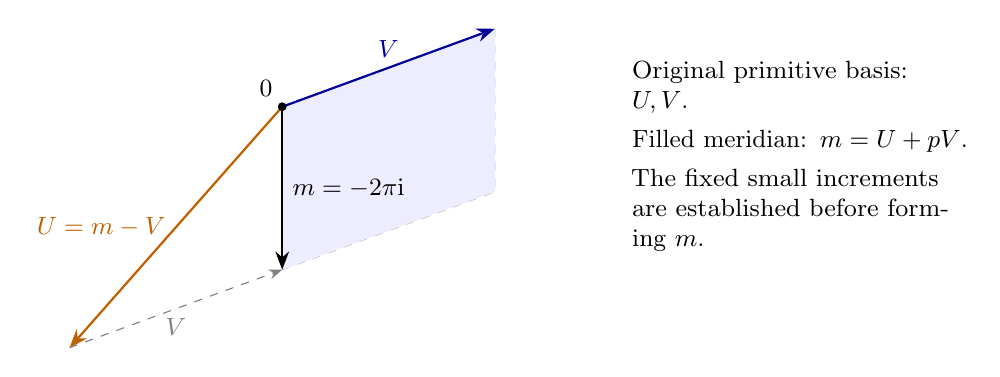
\begin{tikzpicture}[x=.9cm,y=.9cm,>=Stealth,
 every node/.style={font=\small}]
 \coordinate (O) at (0,0); \coordinate (V) at (3,1.1);
 \coordinate (M) at (0,-2.3); \coordinate (U) at (-3,-3.4);
 \draw[gray!55,dashed] (V)--(3,-1.2)--(M);
 \fill[blue!7] (O)--(V)--(3,-1.2)--(M)--cycle;
 \draw[->,thick,blue!60!black] (O)--node[above] {$V$}(V);
 \draw[->,thick] (O)--node[right] {$m=-2\pi\ii$}(M);
 \draw[->,thick,orange!75!black] (O)--node[left] {$U=m-V$}(U);
 \draw[dashed,->,gray] (U)--node[below] {$V$}(M);
 \fill (O) circle (1.6pt); \node[above left] at (O) {$0$};
 \node[align=left,anchor=west,text width=4.2cm] at (4.8,-.7)
 {Original primitive basis: $U,V$.\\[3pt]
  Filled meridian: $m=U+pV$.\\[3pt]
  The fixed small increments are established before forming $m$.};
\end{tikzpicture}

\caption{The developed logarithmic link of a filled original
crossing circle. The old basis is $U,V$, while
$m=U+pV=-2\pi\ii$ is the primitive meridian of the added solid
torus. The picture shows $p=1$; the proof uses the small periods
before multiplying by any integer $p$. In the tube metric,
$m$ makes one angular turn and $V$ gives a nonzero axial
translation.}
\label{sm:period-figure}
\end{figure}

This verifies the metric conclusion of Theorem~\ref{sm:fillings}
for the actual disk-filled exterior. In particular high-index
estimates for a quantum coefficient, source positivity and whole
character-variety rigidity have played no role.

\section{Absolute volume on the original chain}\label{sm:absolute}

Set $G=2\pi\ii\Phi_\eps$. The exact peripheral identity gives
\begin{equation}\label{sm:primitive}
 \dd G=\frac12\sum_i V_i\,\dd U_i,\qquad
 \Ima G(0)=2\pi F_0=\Vol(Y_E^\eps).
\end{equation}
This is the $V\,dU$ polarization. A primitive of
$-\tfrac12\sum U\,dV$ differs by the boundary term
$\tfrac12\sum UV$; its regulator correction cannot be reused
unchanged here.

Let $\mathcal V(\rho)$ be the signed sum of the ideal tetrahedron
volumes of the retained original chain. The local boundary
differential \cite[equation~(7.3)]{Marked} reads, for similarity logs,
\begin{equation}\label{sm:volume-differential}
 \dd\mathcal V
     =\frac12\sum_i\bigl(\Rea V_i\,\dd\Ima U_i
                          -\Rea U_i\,\dd\Ima V_i\bigr).
\end{equation}
Its hypotheses hold on our positive nondegenerate chain:
internal faces cancel by the actual maps, edge-log sums stay fixed,
and the primitive cusp orientation is
$\Ima(\lambda/\mu)>0$ by \eqref{sm:tau}.
All main logs vanish. The proof of that local identity differentiates
Bloch--Wigner volume and cancels normal-face flows; it uses the
positive ordered model $(0,\infty,1,z)$ and the primitive cusp
intersection pairing. It is not a theorem restricted to the
complete packing of a particular diagram.

Taking the imaginary part of \eqref{sm:primitive} and differentiating
its boundary correction now gives
\begin{equation}\label{sm:regulator}
 \mathcal V(\rho_{\boldsymbol\chi})
      =2\pi\Rea\Phi_\eps(\boldsymbol\chi)
                     -\frac12\sum_i\Rea U_i\,\Ima V_i .
\end{equation}
The integration constant is fixed by the actual degree-one complete
cell volumes, not just by a derivative computation.
At a filling solution write $\chi_i=u_i+\ii v_i$. Since
$V_i=2\pi\ii(\chi_i-1)/p_i$,
\begin{equation}\label{sm:boundary-term}
 -\frac12\Rea U_i\,\Ima V_i
    =-\frac{2\pi^2}{p_i}v_i(u_i-1)
    =2\pi\Rea\left[\frac{\pi\ii}{2p_i}(\chi_i-1)^2\right].
\end{equation}
Unfilled auxiliaries have $U_i=V_i=0$.

\subsection{The same boundary triangulation after filling}
It remains to identify $\mathcal V$ with the volume of the smooth
metric just constructed. We verify the chain hypotheses of
\cite[Section~7.3]{Marked}. At a filled cusp conjugate the common
fixed points to $0,\infty$. On each triangle of the retained
boundary triangulation the ideal conical development is
$(a(w),Yb(w))$, with $b>0$. All functions and their derivatives
are bounded on a finite fundamental set. Choose an equivariant
axis map $(0,Y e^{\eta(w)})$, where $\eta$ has the real peripheral
logarithmic character. On the \emph{same} triangulation set
\begin{equation}\label{sm:chain-homotopy}
 H_s(w,Y)=\left(sa(w),
      Y\exp\bigl((1-s)\eta(w)+s\log b(w)\bigr)\right),
                  \qquad 0\le s\le1.
\end{equation}
Both horizontal coordinates and heights have the required
equivariance, and the homotopy agrees along every face.
Its height is comparable to $Y$, horizontal derivatives are bounded,
and height derivatives are $O(Y)$. The volume form
$y^{-3}\,dx_1\wedge dx_2\wedge dy$ therefore bounds its
three-dimensional boundary sweep by $O(Y^{-2})$.

Once the primitive slope is killed, extend that axis-valued boundary
over the added solid torus. The remaining cyclic group acts along
the axis, so all added vertices can lie on the axis and all added
tetrahedra have zero signed volume. At unfilled cusps the same
vanishing boundary estimate applies. Stokes on finite truncations,
followed by $Y\to\infty$, identifies the retained ideal chain with
the filled equivariant fundamental class. Comparing it with the
complete metric developing map on a common subdivision gives
\[
                 \mathcal V(\rho_{\boldsymbol\chi_*})
                        =\Vol(Y_E^\eps(\mathbf p;I)).
\]
An unrelated chain with the same peripheral differential would not
suffice; \eqref{sm:chain-homotopy} supplies the absolute comparison.
Combining it with \eqref{sm:regulator} and
\eqref{sm:boundary-term} proves \eqref{sm:filled-volume}.

\section{Proof boundary and finite algebra}\label{sm:scope}

The strict variational existence, Hessian and boundary-profile
identities are imported from \cite{Profiles}, with their precise
nonmetric content in Section~\ref{sm:variational}. The only local
volume input is the classical ideal-tetrahedron formula
\eqref{sm:tetra}. The local cells, all supporting planes and
cross ratios, entire rational prism maps, collar words and
similarity multipliers are proved here. The individual-mask
induction establishes their enlarged closed topology and every
actual versus completion-map status. The earlier
completed-root papers \cite{Geometry,Fillings} are archival
accounts of that narrower construction, not prerequisites of
the present local calculations or global theorem.
Smooth metric completion and the local
volume differential are the explicitly stated inputs from
\cite{Marked}, with all hypotheses verified here.

No source asymptotic, full spectral bound or nonzero Fourier
contribution is claimed. To identify the classical action with a
quantum packet one must independently match each endpoint-normalized
leaf action, including its color-dependent additive constant, and
then eliminate these same wires. A further whole-source estimate
and filling noncancellation theorem are needed for an invariant
volume limit. The geometry alone does not supply them.
Similarly no equivalence with a completed-root presentation is used,
and no moving main-meridian or preferred-longitude deformation
claim is made.

The accompanying \texttt{check.py} verifies the finite mask closure
and its allowed edge pairings, the literal endpoint-connection
table, projective turn/closing and pure/odd return identities,
the independent-phase prism table, complete collar conjugations,
deformed peripheral multipliers, and the primitive Hessian and
critical boundary normalization.
It includes altered mask, pairing and factor-of-two controls.
It writes a source-hashed JSON record with \texttt{--output}.
These exact finite checks do not prove convexity, the variational
existence theorem, the original manifold identification,
implicit-function theory, smooth completeness or the chain
comparison.

\begin{thebibliography}{9}
\bibitem{Profiles}
\emph{Stationary profiles of strict Newton trees},
companion paper, Lemma~2.2, Theorem~3.3, Lemma~4.1 and
Proposition~4.2.
\href{https://sashakolpakov.github.io/murakamis_dream/papers/strict-newton-profiles.pdf}
{Companion PDF}.

\bibitem{Geometry}
\emph{Pyramids, prisms, and complete geometry of Conway closures},
archival companion for the completed-root grammar.
\href{https://sashakolpakov.github.io/murakamis_dream/papers/conway-geometry.pdf}
{Companion PDF}.

\bibitem{Fillings}
\emph{Marked deformations and long fillings of Conway closures},
archival companion for the completed-root grammar.
\href{https://sashakolpakov.github.io/murakamis_dream/papers/conway-fillings.pdf}
{Companion PDF}.

\bibitem{Marked}
\emph{Circle patterns and primitive fillings of augmented links},
companion paper, Proposition~6.1, equation~(7.3) and Section~7.3.
\href{https://sashakolpakov.github.io/murakamis_dream/papers/marked-fillings.pdf}
{Companion PDF}.

\bibitem{Milnor}
J.~Milnor, Hyperbolic geometry: the first 150 years,
\emph{Bull.\ Amer.\ Math.\ Soc.\ (N.S.)} \textbf{6} (1982), 9--24.
\href{https://doi.org/10.1090/S0273-0979-1982-14958-8}
{doi:10.1090/S0273-0979-1982-14958-8}.

\bibitem{Purcell}
J.~S.~Purcell, An introduction to fully augmented links,
\emph{Contemp.\ Math.} \textbf{541} (2011), 205--220.
\href{https://users.monash.edu.au/~jpurcell/papers/expos-auglinks.pdf}
{Author's manuscript}.

\bibitem{NZ}
W.~D.~Neumann and D.~Zagier, Volumes of hyperbolic three-manifolds,
\emph{Topology} \textbf{24} (1985), 307--332.
\href{https://doi.org/10.1016/0040-9383(85)90004-7}
{doi:10.1016/0040-9383(85)90004-7}.
\end{thebibliography}

\end{document}
